\documentclass[a4paper,11pt,cours]{nsi} % COMPILE WITH DRAFT
\geometry{margin=2cm}
\usepackage[]{fontawesome5}

\setcounter{chapter}{0} % 1 de moins que le num de chapitre
\setlength{\columnseprule}{0pt}

\chapter{Suites numériques,\\ modèles discrets}

\begin{document}

Dans tout ce chapitre, on considère des suites numériques.\\

\section{Définition et représentation graphique d'une suite}
\begin{definition}[ : Suite définie par une formule explicite]
    Définir une suite $(u_n)$ par une formule explicite, c'est donner pour tout entier $n$ l'expression du terme $u_n$ en fonction de $n$.
\end{definition}

\begin{exemple}[]
    La suite $(u_n)$ est définie pour tout $n\in\N$ par $u_n=3n+1$.\\
    On a donc $\quad u_0=3\times 0+1=1\quad$ et $\quad u_{20}=3\times 20+1=61$.
\end{exemple}

\begin{definition}[ : Suite définie par une relation de récurrence]
    Définir une suite par une relation de récurrence, c'est donner un (ou plusieurs) premier(s) terme(s) et une relation permettant de calculer un terme à partir d'un ou plusieurs termes précédents.
\end{definition}

\begin{exemple}[]
    La suite $(v_n)$ est définie par $\left\{
		\begin{array}{llll}
			v_0 & = & -4 & \\
			v_{n+1} & = & 3v_n+1 & \text{pour tout } n\in\N\\
		\end{array}
    \right. $\\
    \begin{multicols}{2}
        \begin{tabbing}
            On a : $\quad v_1$ \=$=3v_0+1$\\
            \>  $=3\times (-4)+1$\\
            \>  $=-11$
        \end{tabbing}
        \begin{tabbing}
            Et : $\quad v_2$  \=$=3v_1+1$\\
            \>  $=3\times (-11)+1$\\
            \>  $=-32$
        \end{tabbing}
    \end{multicols}
\end{exemple}

\newpage

\begin{methode}[ : Modéliser avec une suite]
    \textbf{Un lycée a 1500 élèves inscrits le 1$^{\text{er}}$ septembre 2024. Chaque année, 30 \% des anciens élèves ne se réinscrivent pas et il y a 500 nouveaux élèves.
    \begin{enumerate}
        \item Combien y aura-t-il d'élèves inscrit au lycée le 1$^{\text{er}}$ septembre 2025 ?
        \item Modéliser cette situation à l'aide d'une suite.
    \end{enumerate}}



    \begin{enumerate}
        \item 30 \% des élèves ne se réinscrivent pas. Cela correspond à une baisse de 30 \% : le nombre d'élèves est multiplié par $\left(1-\dfrac{30}{100}\right)$.\\
        $1500\times \left(1-\dfrac{30}{100}\right) +500=1550$.\\
        Il y aura donc 1550 élèves incrits au 1$^{\text{er}}$ septembre 2025.
        \item Pour tout $n\in\N$, on note $u_n$ le nombre d'élèves inscrits au lycée en $2024+n$.\\[.5em]
        $u_0$ est le nombre d'élèves inscrit au lycée au 1$^{\text{er}}$ septembre 2024.\\
        $u_0=1500$\\[.5em]
        Soit $n\in\N$, $u_{n+1}$ est le nombre d'élèves inscrits en $2024+n+1$, c'est-à-dire l'année suivant $2024+n$.
        \begin{tabbing}
            $u_{n+1}$   \=$=u_n\times \left(1-\dfrac{30}{100}\right)+500$\\[.5em]
            \>  $=0,7u_n+500$
        \end{tabbing}
        
    \end{enumerate}
\end{methode}



\subsection*{Représentation graphique d'une suite}
Pour représenter graphiquement la suite $(u_n)$ dans un repère, on place les points de coordonnées $(n\ ;\ u_n)$ avec $n\in\N$.

%\newpage

\begin{exemple}[]
    \dleft{12cm}{
        La suite $(u_n)$ définie pour tout $n\in\N$ par $u_n=2n-1$ est représentée graphiquement dans le repère ci-contre.
    }
    {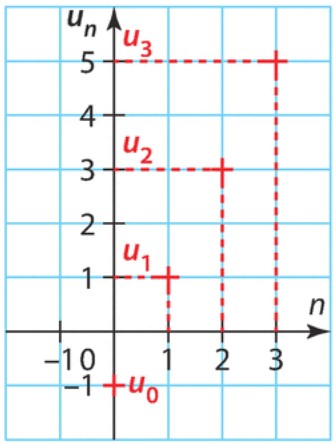
\includegraphics[width=3.5cm]{graphique1.jpg}}
\end{exemple}

\begin{propriete}[s]
    Soient $(u_n)$ une suite réelle et $f$ une fonction.
    \begin{enumerate}[label=\textbullet]
        \item \textbf{Formule explicite :}\\
        Si la suite $(u_n)$ est définie pour tout $n\in\N$ par $u_n=f(n)$, alors $u_n$ est l'ordonnée du point d'abscisse $n$ appartenant à la courbe représentative de la fonction $f$.
        \item \textbf{Relation de récurrence :}\\
        Si la suite $(u_n)$ est définie par donnée de son premier terme $u_0$ et $u_{n+1}=f(u_n)$ pour tout $n\in\N$, alors, on construit graphiquement les termes de la suite à l'aide de la courbe représentative de la fonction $f$ et de la droite d'équation $y=x$ (la première bissectrice).
    \end{enumerate}
\end{propriete}

\setlength{\columnseprule}{0.1pt}

\begin{exemple}[s]
    \begin{multicols}{2}
        la fonction $f$ est définie sur $\fio{0}{+\infty}$ par $f(x)=1+\sqrt{x}$.\\
        La suite $(u_n)$ est définie pour tout $n\in\N$ par $u_n=f(n)$.
        \begin{center}
            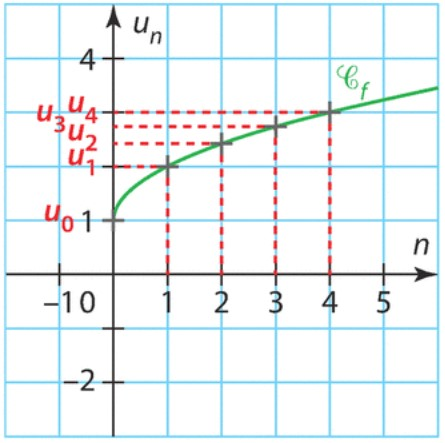
\includegraphics[height=4.5cm]{graphique2.jpg}
        \end{center}
        la fonction $f$ est définie sur $\fio{0}{+\infty}$ par $f(x)=\sqrt{x}$.\\
        La suite $(u_n)$ est définie par\\ $u_0=9$ et $u_{n+1}=f(u_n)$ pour tout $n\in\N$.
        \begin{center}
            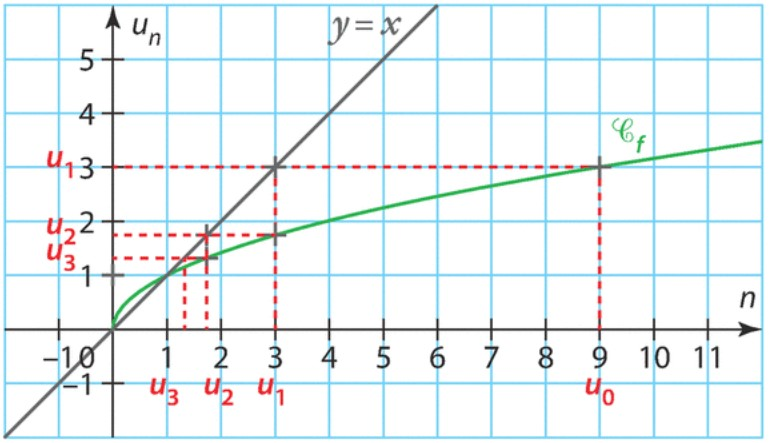
\includegraphics[height=4.5cm]{graphique3.jpg}
        \end{center}
    \end{multicols}
\end{exemple}

\begin{methode}[ : Représenter graphiquement une suite définie par une relation de récurrence]
    \textbf{Représenter graphiquement les 5 premiers termes de la suite $(u_n)$ définie par $$\left\{
		\begin{array}{llll}
			u_0 & = & 6 & \\
			u_{n+1} & = & -\dfrac{1}{2}u_n+2 & \text{pour tout } n\in\N\\
		\end{array}
    \right. $$}
    Pour tout $n\in\N$, on a $\quad u_{n+1}=f(u_n)\quad $ avec $f$ la fonction définie sur $\R$ par $\quad f(x)=-\dfrac{1}{2}x+2$.
    \begin{enumerate}[label=\textbullet]
        \item On commence par tracer la courbe représentative de $f$ (ici la droite verte) et la première bissectrice.
        \item On représente ensuite les termes de la suite un par un :
        \begin{itemize}
            \item On place $u_0$ sur l'axe des abscisses.
            \item Pour obtenir $u_1$, on cherche l'image de $u_0$ par la fonction $f$.
            \item On obtient la valeur de $u_1$ sur l'axe des ordonnées.
            \item On utilise la première bissectrice pour reporter $u_1$ sur l'axe des abscisses.
            \item Pour obtenir $u_2$, on cherhe l'image de $u_1$ par la fonction $f$. On continue ainsi pour obtenir les termes suivants
        \end{itemize}
    \end{enumerate}
    \begin{center}
        \def\xmin{-2} \def\ymin{-2}\def\xmax{7}\def\ymax{4}
        \begin{tikzpicture}[scale=1.5]
            \clip (\xmin,\ymin) rectangle (\xmax,\ymax);
            \draw[fill = white] (\xmin,\ymin) rectangle (\xmax,\ymax);
            \reperenb{\xmin}{\ymin}{\xmax}{\ymax}{$n$}{$u_n$}
            
            \pointcx{6}{-1}{$u_0$}{$u_1$}{}
            \pointcx{-1}{-1}{}{}{}
            \pointcx{-1}{2.5}{$u_1$}{$u_2$}{}
            \pointcx{2.5}{2.5}{}{}{}
            \pointcx{2.5}{.75}{$u_2$}{$u_3$}{}
            \pointcx{.75}{.75}{}{}{}
            \pointcx{.75}{1.625}{$u_3$}{$u_4$}{}
            \pointcx{1.625}{1.625}{$u_4$}{}{}

            \draw[thick,UGLiDarkGreen,domain=\xmin:\xmax,smooth,variable=\x] plot ({\x},{-0.5*\x+2});
            \draw[thick,UGLiRed,domain=\xmin:\xmax,smooth,variable=\x] plot ({\x},{\x});
        \end{tikzpicture}
    \end{center}
    
\end{methode}

\subsection*{Utilisation de la calculatrice}
\dleft{14cm}{Tutoriels vidéos pour utiliser l'application « Suites » de la calculatrice : }{
\includegraphics[width=2cm]{code-qr1.png}}

\section{Suites de références}
\subsection*{Suites arithmétiques}
\begin{definition}[ ]
	Une suite $(u_n)$ est dite \textbf{arithmétique} s'il existe un nombre réel $r$ tel que pour tout entier $n$ on a $u_{n+1}=u_n+r$ \hspace{.5cm}(relation de récurrence).\\
	Le nombre $r$ est appelé \textbf{raison} de la suite $(u_n)$.
\end{definition}

\begin{propriete}[ ]
	Si $(u_n)$ est une suite \textbf{arithmétique} de raison $r$, alors pour tous entiers naturels $n$ et $p$ :
	\begin{enumerate}[label=\textbullet]
		\item 	$u_n = u_0+n\times r$ \hspace{.5cm}(forme explicite)
		\item 	$u_n=u_p+(n-p)r$	
    \end{enumerate}
\end{propriete}

\begin{exemple}[ : Représentation graphique d'une suite arithmétique]
    \dleft{9.5cm}{On a représenté ci-contre les premiers termes de la suite définie pour tout $n\in\N$ par :\\[.5em]
    .\dotfill\\
    
    Les points représentant les termes de cette suite sont alignés sur la droite d'équation réduite\\[.5em]
    .\dotfill}
    {\begin{center}
        \def\xmin{-1} \def\ymin{-2}\def\xmax{5}\def\ymax{12}
        \begin{tikzpicture}[yscale=.5]
            \clip (\xmin,\ymin) rectangle (\xmax,\ymax);
            \draw[fill = white] (\xmin,\ymin) rectangle (\xmax,\ymax);
            \reperenb{\xmin}{\ymin}{\xmax}{\ymax}{$n$}{$u_n$}
            \draw 	(0,1)	\ball node[above left]{$A_0$} (1,4)	\ball node[above left]{$A_1$}
            (2,7)	\ball node[above left]{$A_2$} (3,10) \ball node[above left]{$A_3$};
            \coordinate (A) at (0,0);

            \draw[ultra thick,UGLiRed,->,>=stealth] (0,1) -- node[below]{$+1$} (1,1) ;
            \draw[ultra thick,UGLiRed,->,>=stealth] (1,4) -- node[below]{$+1$} (2,4) ;
            \draw[ultra thick,UGLiRed,->,>=stealth] (2,7) -- node[below]{$+1$} (3,7) ;

            \draw[ultra thick,UGLiOrange,->,>=stealth] (1,1) -- node[right]{$+r$} (1,4) ;
            \draw[ultra thick,UGLiOrange,->,>=stealth] (2,4) -- node[right]{$+r$} (2,7) ;
            \draw[ultra thick,UGLiOrange,->,>=stealth] (3,7) -- node[right]{$+r$} (3,10) ;

            \draw[dashed,domain=0:\xmax,smooth,variable=\x] plot ({\x},{3*\x+1});
        \end{tikzpicture}
    \end{center}}
\end{exemple}

\begin{propriete}[]
    Pour tout entier naturel $n\geqslant1, \quad 1+2+...+n=\dfrac{n(n+1)}{2}$.
\end{propriete}

\begin{propriete}[ : Somme des termes d'une suite arithmétique]
	Soit $(u_n)$ une suite arithmétique de raison $r$ et de premier terme $u_0$.\\
	Soient $n$ et $p $ deux entiers naturels, avec $n<p$.
	\begin{enumerate}[label=\textbullet]
		\item La somme des $n+1$ premiers termes de la suite $u_n$ est égale à :
		$$u_0+u_1+u_2+...u_{n-1}+u_n=(n+1)\dfrac{u_0+u_n}{2}$$
		\item La somme des termes d'indice $p$ à $n$ est égale à :
		$$u_p+u_{p+1}+...+u_n=(n-p+1)\dfrac{u_p+u_n}{2}$$
	\end{enumerate}
\end{propriete}

%\newpage
\subsection*{Suites géométriques}

\begin{definition}[ ]
	Une suite $(u_n)$ est dite \textbf{géométrique} s'il existe un nombre réel $q$ tel que pour tout entier $n$ on a $u_{n+1}=q \times u_n$ \hspace{.5cm}(relation de récurrence).\\
	Le nombre $q$ est appelé \textbf{raison} de la suite $(u_n)$.
\end{definition}

\begin{propriete}[ ]
	Si $(u_n)$ est une suite \textbf{géométrique} de raison $q\neq 0$, alors pour tous entiers naturels $n$ et $p$ :
	\begin{enumerate}[label=\textbullet]
		\item 	$u_n = u_0\times q^n $  \hspace{.5cm}(forme explicite)
		\item 	$u_n=u_p\times q^{n-p}$	
	\end{enumerate}
\end{propriete}

\begin{propriete}[]
    Pour tout réel $q\neq 1$ et pour tout entier naturel $n, \quad 1+q+q^2+...+q^n=\dfrac{1-q^{n+1}}{1-q}$.
\end{propriete}

\begin{propriete}[ : Somme des termes d'une suite géométrique]
	Soit $(u_n)$ une suite géométrique de raison $q\neq 1$ et de premier terme $u_0$.\\
	Soient $n$ et $p $ deux entiers naturels, avec $n<p$.
	\begin{enumerate}[label=\textbullet]
		\item La somme des $n+1$ premiers termes de la suite $u_n$ est égale à :
		$$u_0+u_1+u_2+...u_{n-1}+u_n=u_0\times \dfrac{1-q^{n+1}}{1-q}$$
		\item La somme des termes d'indice $p$ à $n$ est égale à :
		$$u_p+u_{p+1}+...+u_n=u_p\times \dfrac{1-q^{n-p+1}}{1-q}$$
	\end{enumerate}
\end{propriete}

\section{Limite d'une suite}
\begin{definition}[ : Limite réelle d'une suite]
    Soient $(u_n)$ une suite et $l$ un nombre réel.\\
    La suite $(u_n)$ a pour \textbf{limite} $l$ lorsque $n$ tend vers $+\infty$, si les termes $u_n$ deviennent aussi proches de $l$ que l'on veut quand $n$ est suffisamment grand.\\[.5em]
    On dit que \textbf{$(u_n)$ converge vers $l$} et on note $\quad\lim\limits_{n\to+\infty}u_n=l$.
\end{definition}

\begin{exemple}[]
    $(u_n)$ est la suite définie sur $\N^*$ par $\quad u_n=\dfrac{1}{n}+1$.
    \begin{center}
        \def\xmin{-1} \def\ymin{-2}\def\xmax{11}\def\ymax{3}
        \begin{tikzpicture}[scale=0.7]
            \clip (\xmin,\ymin) rectangle (\xmax,\ymax);
            \draw[fill = white] (\xmin,\ymin) rectangle (\xmax,\ymax);
            \reperenb{\xmin}{\ymin}{\xmax}{\ymax}{$n$}{$u_n$}
            \draw 	 (1,2) \ball (2,1.5)	\ball (3,1.33) \ball (4,1.25) \ball  (5,1.2) \ball (6,1.167)	\ball (7,1.14) \ball (8,1.125) \ball  (9,1.11) \ball (10,1.1) \ball;
            \draw[UGLiDarkGreen,thick,dashed,domain=0:\xmax,smooth,variable=\x] plot ({\x},{1});
    
        \end{tikzpicture}
    \end{center}
    Il semble que $u_n$ est aussi proche de $1$ que l'on veut lorsque $n$ est suffisamment grand.\\
    La suite $(u_n)$ a pour limite $1$. On note : $\quad \lim\limits_{n\to+\infty} u_n=1$.
\end{exemple}


\begin{definition}[ : Limite infinie d'une suite]
    Soit $(u_n)$ une suite.\\
    La suite $(u_n)$ a pour \textbf{limite} $+\infty$ (respectivement $-\infty$) lorsque $n$ tend vers $+\infty$, si les termes $u_n$ deviennent aussi grands (respectivement petits) que l'on veut quand $n$ est suffisamment grand.\\[.5em]
    On dit que \textbf{$(u_n)$ diverge} et on note $\quad\lim\limits_{n\to+\infty}u_n=+\infty\quad$ (respectivement $\quad\lim\limits_{n\to+\infty}u_n=-\infty$).
\end{definition}

\begin{exemple}[]
    $(v_n)$ est la suite définie sur $\N$ par $\quad v_n=-0,5 n^2$.
    \begin{center}
        \def\xmin{-1} \def\ymin{-80}\def\xmax{11}\def\ymax{20}
        \begin{tikzpicture}[xscale=.7,yscale=0.035]
            \tikzstyle{every node}=[font=\small]


            \clip (\xmin,\ymin) rectangle (\xmax,\ymax);
            \draw[fill = white] (\xmin,\ymin) rectangle (\xmax,\ymax);
            
            %\draw 	(0,4)	\ball node[above left]{$A_0$} (1,2)	\ball node[above left]{$A_1$}    (2,1)	\ball node[above left]{$A_2$} (3,0.5) \ball node[above left]{$A_3$} (4,0.25) \ball node[above left]{$A_4$} (5,0.125) \ball node[above left]{$A_5$} (6,0.0625) \ball node[above left]{$A_6$};
            \draw[->] (\xmin,0) -- (\xmax,0);
            \draw[UGLiBlue, domain=\xmin:\xmax,variable=\x] plot({\x},{-20});
            \draw[UGLiBlue, domain=\xmin:\xmax,variable=\x] plot({\x},{-40});
            \draw[UGLiBlue, domain=\xmin:\xmax,variable=\x] plot({\x},{-60});
           
            
            %\draw[UGLiRed,domain=0:\xmax,smooth,variable=\x] plot ({\x},{35*1.03^(10*\x)});
           
            %\draw[ UGLiBlue] (-0.5,\ymin) -- (-0.5,\ymax);
            \draw[->] (0,\ymin) -- (0,\ymax);
            \draw[ UGLiBlue] (1,\ymin) -- (1,\ymax);
            \draw[ UGLiBlue] (2,\ymin) -- (2,\ymax);
            \draw[ UGLiBlue] (3,\ymin) -- (3,\ymax);
            \draw[ UGLiBlue] (4,\ymin) -- (4,\ymax);
            \draw[ UGLiBlue] (5,\ymin) -- (5,\ymax);
            \draw[ UGLiBlue] (6,\ymin) -- (6,\ymax);
            \draw[ UGLiBlue] (7,\ymin) -- (7,\ymax);
            \draw[ UGLiBlue] (8,\ymin) -- (8,\ymax);
            \draw[ UGLiBlue] (9,\ymin) -- (9,\ymax);
            \draw[ UGLiBlue] (10,\ymin) -- (10,\ymax);

            \draw (0,0) node[below left] {$0$} (0,-20) node[below left] {$-20$} (0,-40) node[below left] {$-40$} (0,-60) node[below left] {$-60$} (0,20) node[below right] {$v_n$};

            \draw (1,0) node[above ] {$1$} (2,0) node[above] {$2$} (3,0) node[above ] {$3$} (4,0) node[above] {$4$} (5,0) node[above] {$5$} (6,0) node[above] {$6$} (7,0) node[above] {$7$} (8,0) node[above] {$8$} (9,0) node[above] {$9$} (10,0) node[above] {$10$} (11,0) node[below left] {$n$};

            \draw[] (0,0) \ball (1,-.5) \ball (2,-2) \ball (3,-4.5) \ball (4,-8) \ball (5,-12.5) \ball (6,-18) \ball (7,-24.5) \ball (8,-32) \ball (9,-40.5) \ball (10,-50) \ball;
        \end{tikzpicture}
    \end{center}
    Il semble que $v_n$ est aussi petit que l'on veut lorsque $n$ est suffisamment grand.\\
    La suite $(v_n)$ a pour limite $-\infty$. On note : $\quad \lim\limits_{n\to+\infty} v_n=-\infty$.
\end{exemple}

\begin{remarque}[]
    Une suite \textbf{diverge} lorsqu'elle n'a pas de limite finie.\\
    Une suite \textbf{divergente} n'admet pas nécessairement de limite infinie.
\end{remarque}


\begin{exemple}[]
    La suite $(t_n)$ définie sur $\N$ par $t_n=(-1)^n$ n'a pas de limite : ses termes valent alternativement $1$ et $-1$.
    \begin{center}
        \def\xmin{-1} \def\ymin{-2}\def\xmax{11}\def\ymax{2}
        \begin{tikzpicture}[scale=0.7]
            \clip (\xmin,\ymin) rectangle (\xmax,\ymax);
            \draw[fill = white] (\xmin,\ymin) rectangle (\xmax,\ymax);
            \reperenb{\xmin}{\ymin}{\xmax}{\ymax}{$n$}{$t_n$}
            \draw 	(0,1) \ball  (1,-1) \ball (2,1)	\ball (3,-1) \ball (4,1) \ball  (5,-1) \ball (6,1)	\ball (7,-1) \ball (8,1) \ball  (9,-1) \ball (10,1) \ball;

    
        \end{tikzpicture}
    \end{center}
    $(t_n)$ est une suite divergente.
\end{exemple}


\newpage

\subsection*{Limite des suites de référence}
\begin{propriete}[]
    Soit $k\in\N^*$.
    \begin{enumerate}[label=\textbullet]
        \item Les suites $(\sqrt{n}), (n)$ et $(n^k)$ ont pour limite $+\infty$.
        \item Les suites $\left(\dfrac{1}{\sqrt{n}}\right), \left(\dfrac{1}{n}\right) $ et $\left(\dfrac{1}{n^k}\right)$ ont pour limite $0$.
    \end{enumerate}
\end{propriete}

\section{Propriétés des limites}
\begin{propriete}[ : Limite d'une somme]
    Soient $(u_n)$ et $(v_n)$ deux suites et $l$ et $l'$ deux nombres réels.\\[.5em]
    \tabstyle[UGLiRed]
    \begin{tabular}{|c|c|c|c|c|c|c|}
    \hline
    \ccell Si $\lim\limits_{n \to+\infty} u_n=...$& $l$ & $l$ & $l$ &$+\infty$ & $+\infty$ & $-\infty$ \\\hline
    \ccell et si $\lim\limits_{n \to+\infty}v_n=...$& $l'$ & $+\infty$ & $-\infty$ &$+\infty$ & $-\infty$ & $-\infty$ \\\hline
    \ccell alors $\lim\limits_{n \to+\infty} (u_n+v_n)=...$& $l+l'$ & $+\infty$ & $-\infty$ &$+\infty$ & \textbf{FI} & $-\infty$ \\\hline
    \end{tabular}

    Dans le cas noté \textbf{FI} (forme indéterminée), on ne peut pas conclure.
\end{propriete}

%\newpage

\begin{exemple}[]
    On veut déterminer la limite de la suite $(u_n)$ définie sur $\N$ par $u_n=n^2+ \dfrac{1}{n}$.\\[.5em]
    On a : $\qquad \lim\limits_{n\to+\infty} n^2=+\infty\qquad$ et $\qquad \lim\limits_{n\to+\infty} \dfrac{1}{n} = 0$\\[.5em]
    Donc $\qquad \lim\limits_{n\to+\infty} u_n=+\infty$.
\end{exemple}

\begin{propriete}[ : Limite d'un produit]
    Soient $(u_n)$ et $(v_n)$ deux suites et $l$ et $l'$ deux nombres réels.\\[.5em]
    \tabstyle[UGLiRed]
    \begin{tabular}{|c|c|c|c|c|c|c|c|c|c|}
    \hline
    \ccell Si $\lim\limits_{n \to+\infty} u_n=...$& $l$ & $l>0$ & $l>0$ & $l<0$ & $l<0$ & $+\infty$ & $+\infty$ & $-\infty$ &$0$ \\\hline
    \ccell et si $\lim\limits_{n \to+\infty}v_n=...$& $l'$ & $+\infty$ & $-\infty$ & $+\infty$ & $-\infty$ &$+\infty$ & $-\infty$ & $-\infty$ & \footnotesize{$+\infty$ ou $-\infty$} \\\hline
    \ccell alors $\lim\limits_{n \to+\infty}(u_n \times v_n) =...$& $l\times l'$ & $+\infty$ & $-\infty$ & $-\infty$ & $+\infty$ & $+\infty$  & $-\infty$ & $+\infty$ & \textbf{FI}\\\hline
    \end{tabular}

    Dans le cas noté \textbf{FI} (forme indéterminée), on ne peut pas conclure.
\end{propriete}

%\newpage

\begin{exemple}[]
    On veut déterminer la limite de la suite $(v_n)$ définie sur $\N$ par $v_n=-5\sqrt{n}-n^3$.\\[.5em]
    On a : $\qquad \lim\limits_{n\to+\infty} \sqrt{n}=+\infty\qquad$ et $\qquad \lim\limits_{n\to+\infty} -5 = -5 \qquad$ donc $\lim\limits_{n\to+\infty} -5\sqrt{n}=-\infty$\\[.5em]
    De plus $\qquad \lim\limits_{n\to+\infty} n^3=+\infty \qquad$ donc $\qquad \lim\limits_{n\to+\infty} -n^3=-\infty$.\\[.5em]
    Donc $\qquad \lim\limits_{n\to+\infty} v_n=+\infty$.
\end{exemple}

\begin{propriete}[ : Limite d'un quotient]
    Soient $(u_n)$ et $(v_n)$ deux suites avec pour tout $n\in\N, v_n\neq 0$ et $l$ et $l'$ deux nombres réels.
    \begin{enumerate}[label=\textbullet]
        \item Cas où $\lim\limits_{n \to+\infty}v_n \neq 0$\\[.5em]
        \tabstyle[UGLiRed]
    \begin{tabular}{|c|c|c|c|c|c|c|c|}
    \hline
    \ccell Si $\lim\limits_{n \to+\infty} u_n=...$& $l$ & $l$ & $+\infty$ & $+\infty$ & $-\infty$ & $-\infty$ & $+\infty$ ou $-\infty$\\\hline
    \ccell et si $\lim\limits_{n \to+\infty}v_n=...$& $l'\neq 0$ & $+\infty$ ou $-\infty$ & $l'>0$ &$l'<0$ & $l'>0$ &$l'<0$ & $+\infty$ ou $-\infty$ \\\hline
    \ccell alors $\lim\limits_{n \to+\infty} \dfrac{u_n}{v_n}=...$& $\dfrac{l}{l'}$ & $0$ & $+\infty$ &$-\infty$ & $-\infty$ & $+\infty$ & \textbf{FI}  \\\hline
    \end{tabular}
        \item Cas où $\lim\limits_{n \to+\infty}v_n = 0$\\[.5em]
        \tabstyle[UGLiRed]
    \begin{tabular}{|c|p{2cm}|p{2cm}|p{2cm}|p{2cm}|c|}
    \hline
    \ccell Si $\lim\limits_{n \to+\infty} u_n=...$& \small{$l>0$ ou $+\infty$} & \small{$l<0$ ou $-\infty$} & \small{$l>0$ ou $+\infty$} & \small{$l<0$ ou $-\infty$} & $\quad 0 \quad$\\\hline
    \ccell et si $\lim\limits_{n \to+\infty}v_n=...$& $0$ en restant positif & $0$ en restant positif & $0$ en restant négatif & $0$ en restant négatif & $0$\\\hline
    \ccell alors $\lim\limits_{n \to+\infty} \dfrac{u_n}{v_n}=...$ & $\qquad +\infty$ &$\qquad -\infty$ & $\qquad -\infty$ & $\qquad +\infty$ & \textbf{FI}  \\\hline
    \end{tabular}
    \end{enumerate}

    Dans les cas notés \textbf{FI} (forme indéterminée), on ne peut pas conclure.
\end{propriete}

\begin{exemple}[]
    On veut déterminer la limite de la suite $(w_n)$ définie sur $\N$ par $w_n=\dfrac{2}{3n+5}$.\\[.5em]
    On a : $\qquad \lim\limits_{n\to+\infty} 2=2\qquad$ et $\qquad \lim\limits_{n\to+\infty} 3n+5 = +\infty \qquad$ (par produit et par somme).\\[.5em]
    Donc $\qquad \lim\limits_{n\to+\infty} w_n=0$.
\end{exemple}

\begin{methode}[ : Lever une forme indéterminée]
    On veut calculer la limite de la suite $(t_n)$ définie sur $\N$ par $\quad t_n=n^2-n$.\\

    On a : $\qquad \lim\limits_{n\to+\infty} n^2=+\infty\qquad$ et $\qquad \lim\limits_{n\to+\infty} n=+\infty$.\\[.5em]
    On obtient donc une forme indéterminée « $+\infty-\infty$ ».\\

    \faLightbulb \hspace*{.3cm} Pour lever l'indétermination, on écrit le terme $t_n$ sous forme \textbf{factorisée}.\\
    Pour tout $n\in\N, \quad t_n=n(n-1)$.\\[.5em]
    On a : $\qquad \lim\limits_{n\to+\infty} n=+\infty\qquad$ et $\qquad \lim\limits_{n\to+\infty} (n-1)=+\infty$.\\[.5em]
    Donc $\qquad \lim\limits_{n\to+\infty} t_n=+\infty \qquad$ (par produit).
\end{methode}


\section{Limites et comparaisons}
\begin{encadrecolore}{Théorème de comparaison}{UGLiRed}
    Soient $(u_n)$ et $(v_n)$ deux suites.\\
    On suppose qu'il existe un entier $n_0$ tel que pour tout $n\geqslant n_0, \quad u_n\leqslant v_n$.
    \begin{enumerate}[label=\textbullet]
        \item Si $\ \lim\limits_{n\to+\infty}u_n=+\infty\quad$ alors $\quad \lim\limits_{n\to+\infty}v_n=+\infty$.
        \item Si $\ \lim\limits_{n\to+\infty}v_n=-\infty\quad$ alors $\quad \lim\limits_{n\to+\infty}u_n=-\infty$.
    \end{enumerate}
\end{encadrecolore}

\begin{exemple}[ d'application]
    Soit $(u_n)$ la suite définie sur $\N$ par $\quad u_n=n+2\sin(n)$.\\
    On cherche à calculer la limite de $(u_n)$.\\

    Pour tout réel $x, \quad -1\leqslant \sin(x)\leqslant 1\quad$ donc pour tout $n\in\N, \quad -1\leqslant \sin(n)\leqslant 1$.\\[.5em]
    Ainsi, pour tout $n\in\N, \quad -2\leqslant 2\sin(n)\leqslant 2\quad$ et $\quad n-2\leqslant n+2\sin(n)\leqslant n+2$.\\[.5em]
    En particulier, pour tout $n\in\N, \quad u_n\geqslant n-2$.\\[.5em]
    Or, $\quad \lim\limits_{n\to+\infty} n-2 =+\infty$.\\[.5em]
    Donc, d'après le théorème de comparaison, $\quad \lim\limits_{n\to+\infty} u_n =+\infty$.
\end{exemple}

%\newpage


\begin{encadrecolore}{Théorème des gendarmes}{UGLiRed}
    Soient $(u_n), (v_n)$ et $(w_n)$ trois suites et $l$ un nombre réel.\\[.5em]
    Si :
    \begin{enumerate}[label=\textbullet]
        \item il existe un entier naturel $n_0$ tel que tout tout entier $n\geqslant n_0, \quad v_n\leqslant u_n \leqslant w_n$ ;
        \item les suites $(v_n)$ et $(w_n)$ convergent vers $l$.
    \end{enumerate}
    Alors la suite $(u_n)$ converge et $\quad \lim\limits_{n\to+\infty}u_n=l$.
\end{encadrecolore}

\begin{exemple}[ d'utilisation]
    Soit $(v_n)$ la suite définie sur $\N^*$ par $\quad v_n=3+\dfrac{(-1)^n}{n}$.\\
    On cherche à déterminer la limite de $(v_n)$.\\

    On ne peut pas déterminer directement la limite de la suite $(v_n)$ en utilisant les propriétés car la suite $\left((-1)^n\right)$ n'a pas de limite.\\
    \faLightbulb \hspace*{.3cm} On encadre la suite $(v_n)$ par deux suites dont on peut déterminer les limites.\\

    Soit $n\in\N^*$.\\
    $-1\leqslant (-1)^n \leqslant 1 \qquad$ donc $\qquad -\dfrac{1}{n} \leqslant \dfrac{(-1)^n}{n} \leqslant \dfrac{1}{n} \qquad$ et $\qquad 3-\dfrac{1}{n} \leqslant v_n \leqslant 3+\dfrac{1}{n}$.\\[.5em]
    Or $\qquad \lim\limits_{n\to+\infty} 3-\dfrac{1}{n}=3\qquad$ et $\qquad \lim\limits_{n\to+\infty} 3+\dfrac{1}{n}=3$.\\[.5em]
    Donc, d'après le théorème des gendarmes, $\quad \lim\limits_{n\to+\infty} v_n=3$.
\end{exemple}

\section{Limites et suites géométriques}
\begin{propriete}[ : Limite de $q^n$]
    Soit $q$ un nombre réel positif ou nul.
    \begin{enumerate}[label=\textbullet]
        \item Si $0\leqslant q < 1, \quad$ alors $\quad \lim\limits_{n\to+\infty} q^n=0$.
        \item Si $ q > 1, \quad$ alors $\quad \lim\limits_{n\to+\infty} q^n=+\infty$.
        \item Si $ q =1, \quad$ alors $\quad \lim\limits_{n\to+\infty} q^n=1$.
    \end{enumerate}
\end{propriete}

\begin{exemple}[]
    $0\leqslant \dfrac{1}{2} <1, \quad$ donc $\quad \lim\limits_{n\to+\infty}\left(\dfrac{1}{2}\right)^n = 0$.
\end{exemple}

\begin{propriete}[ : Limite d'une suite géométrique]
    Soit $(u_n)$ une suite géométrique de raison $q\geqslant 0$ et de premier terme $u_p$ avec $p\in\N$.
    \begin{enumerate}[label=\textbullet]
        \item Si $0\leqslant q<1, \quad$ alors $\quad \lim\limits_{n\to+\infty} u_n=0$.
        \item Si $ q>1$ et $u_p>0, \quad$ alors $\quad \lim\limits_{n\to+\infty} u_n=+\infty$.
        \item Si $ q>1$ et $u_p<0, \quad$ alors $\quad \lim\limits_{n\to+\infty} u_n=-\infty$.
        \item Si $ q=1,\quad$ alors $\quad \lim\limits_{n\to+\infty} u_n=u_p$.
    \end{enumerate}
\end{propriete}

\begin{exemple}[]
    Soit $(u_n)$ la suite définie sur $\N$ par $\left\{
		\begin{array}{llll}
			u_0 & = & 5 & \\
			u_{n+1} & = & \dfrac{u_n}{3} & \text{pour tout } n\in\N\\
		\end{array}
    \right. $\\
    $(u_n)$ est une suite géométrique de raison $\dfrac{1}{3}$.\\
    Or $0\leqslant \dfrac{1}{3}<1,\quad$ donc $\quad \lim\limits_{n\to+\infty} u_n=0$.
\end{exemple}

\begin{propriete}[ : Limite de la somme des termes d'une suite géométrique]
    Soit $(u_n)$ une suite géométrique de premier terme $u_p$ avec $p\in\N$ et de raison $q$ avec $0\leqslant q < 1$.\\
    Pour $n\in\N$, on appelle $S_n$ la somme des $n$ premiers termes de la suite $(u_n)$.\\[.5em]
    On a $\quad \lim\limits_{n\to+\infty} S_n=\dfrac{u_p}{1-q}$.
\end{propriete}

\begin{demonstration}
    Soit $n\in\N$
    \begin{tabbing}
        $S_n$   \= $=u_p+u_{p+1}+u_{p+2}+...+u_{p+n-1}$\\[.5em]
            \> $=u_p + u_p\times q + u_p\times q^2 +... + u_p\times q^{n-1}$\\[.5em]
            \> $=u_p\times \left(1+q+q^2+...+q^{n-1}\right)$\\[.5em]
            \> $=u_p\times \dfrac{1-q^n}{1-q}$
    \end{tabbing}
    On a $\quad 0\leqslant q <1, \quad$ donc $\quad \lim\limits_{n\to+\infty} q^n=0$.\\[.5em]
    Donc $\quad \lim\limits_{n\to+\infty} 1-q^n=1 \quad$ et $\quad \lim\limits_{n\to+\infty} \dfrac{1-q^n}{1-q}=\dfrac{1}{1-q}$.
    \begin{tabbing}
        Ainsi $\quad \lim\limits_{n\to+\infty} S_n$ \=$=u_p\times \dfrac{1}{1-q}$\\[.5em]
        \>$=\dfrac{u_p}{1-q}$
    \end{tabbing}
\end{demonstration}

\begin{exemple}[]
    Soit $(u_n)$ la suite définie sur $\N$ par $\left\{
		\begin{array}{llll}
			u_0 & = & 5 & \\
			u_{n+1} & = & \dfrac{u_n}{3} & \text{pour tout } n\in\N\\
		\end{array}
    \right. $\\
    On a vu précédemment que $(u_n)$ est une suite géométrique de raison $\dfrac{1}{3}$.\\[.5em]
    Pour tout $n\in\N$, on note $S_n$ la somme des $n$ premiers termes consécutifs de la suite $(u_n)$.\\
    $0\leqslant \dfrac{1}{3}<1$ donc suite $(S_n)$ converge.
    \begin{tabbing}
        $\lim\limits_{n\to+\infty}S_n$  \= $=\dfrac{5}{1-\dfrac{1}{3}}$\\[.5em]
            \>  $=\dfrac{5}{\dfrac{2}{3}}$\\[.5em]
            \>  $=5\times \dfrac{3}{2}$\\[.5em]
            \>  $=7,5$
    \end{tabbing}
    
\end{exemple}

\section{Suites arithmético-géométriques}
\begin{definition}[]
    Une suite $(u_n)$ est \textbf{arithmético-géométrique} s'il existe deux nombres réels $a$ et $b$ tels que, pour tout $n\in \N, \quad u_{n+1}=a\ u_n+b$.
\end{definition}

\begin{remarque}[s]
    Soient $a$ et $b$ deux réels tels que pour tout $n\in\N, \quad u_{n+1}=a\ u_n+b$.
    \begin{enumerate}[label=\textbullet]
        \item Si $a=0$, la suite $(u_n)$ est constante à partir du rang 1.
        \item Si $a=1$, la suite $(u_n)$ est arithmétique de raison $b$.
        \item Si $b=0$, la suite $(u_n)$ est géométrique de raison $a$.
    \end{enumerate}
\end{remarque}

\begin{propriete}[ : Suite géométrique associée à une suite arithmético-géométrique]
    Soient $a$ et $b$ deux nombres réels avec $a\neq 1$ et $b\neq 0$.\\
    Soit $(u_n)$ une suite arithmético-géométrique de premier terme $u_p$ ($p\in\N$) telle que pour tout $n\geqslant p, \quad u_{n+1}=a\ u_n+b$.\\
    Soit $l$ le réel tel que $\quad l=al+b$.\\

    La suite $(v_n)$ définie pour tout entier $n\geqslant p$ par $\quad v_n=u_n-l\quad$ est une suite géométrique de raison $a$ et de premier terme $v_p=u_p-l$.
\end{propriete}

\begin{demonstration}
    Soit $n\in\N, n\geqslant p$.
    \begin{tabbing}
        $v_{n+1}$   \= $=u_{n+1}-l$\\
            \>  $= a\ u_n+b -(al+b)$\\
            \>  $= a\ u_n +b -al -b$\\
            \>  $= a(u_n-l)$\\
            \>  $= a\ v_n$
    \end{tabbing}
    $(v_n)$ est donc une suite géométrique de raison $a$.
\end{demonstration}

\begin{methode}[ : Étudier une suite arithmético-géométrique]
    Soit $(u_n)$ la suite définie sur $\N$ par $\left\{
		\begin{array}{llll}
			u_0 & = & 6 & \\
			u_{n+1} & = & 3 u_n-4 & \text{pour tout } n\in\N\\
		\end{array}
    \right. $\\
    On cherche à déterminer l'expression de $u_n$ en fonction de $n$.\\[.5em]
    $(u_n)$ est une suite arithmético-géométrique (ici $a=3$ et $b=-4$).
    \begin{enumerate}[label=\textbullet]
        \item 
        \textbf{On commence par déterminer la suite constante vérifiant la relation de récurrence :}\\ 
        On résout l'équation $x=ax+b$.\\
        Soit $x\in\R$
        \begin{tabbing}
            $x=3x-4 \quad$ \= $\iff \quad -2x=-4$\\
                \> $\iff \quad x=2$
        \end{tabbing}
        La suite constante $(c_n)$ égale à $2$ vérifie la relation $\quad c_{n+1} = 3 c_n-4 \quad  \text{pour tout } n\in\N$.

        \item \textbf{On étudie la suite géométrique auxiliaire :}\\
        On définit la suite $(v_n)$ sur $\N$ par $v_n= u_n-c_n$.\\[.5em]
        Montrons que $(v_n)$ est une suite géométrique :
        \begin{tabbing}
            Soit $n\in\N. \qquad v_{n+1}$ \=$=u_{n+1}-c_{n+1}$\\
            \>  $=3u_n-4-\left(3c_n-4\right)$\\
            \>  $=3\left(u_n-c_n\right)$\\
            \>  $=3\ v_n$
        \end{tabbing}
        
        $(v_n)$ est donc une suite géométrique de raison $3$ et de premier terme $v_0= u_0-2=6-2=4$.
        \begin{tabbing}
            Donc pour tout $n\in\N, \quad v_n$  \=$=v_0\times 3^n$\\
                \>  $=4\times 3^n$
        \end{tabbing}
        
        \item \textbf{On exprime $u_n$ en fonction de $n$ :}
        \begin{tabbing}
            Ainsi, pour tout $n\in\N, \quad u_n$ \= $=v_n+c_n$\\
                \>  $=4\times 3^n+2$
        \end{tabbing}

        \item \textbf{On peut en déduire la limite de $(u_n)$}\\
        $\lim\limits_{n\to+\infty} 3^n=+\infty\qquad$ donc $\qquad \lim\limits_{n\to+\infty} u_n=+\infty \qquad$ (d'après les propriétés sur les limites)
    \end{enumerate}
\end{methode}
\end{document}